\section{Fusion summary}

The Z-Score fusion and regression fusion was shown to improve rank lists quality when fusing good rank list together.

The rank lists obtained by fusing with the Z-Score method every retained rank lists are referred as \textit{Z-Score rank lists}.
This corresponds to one rank list for each corpus.

When fusing rank lists with the regression, fusion pairs of corpora are required (one for training and one for testing).
When evaluating this method with 4 corpora (Oxquarry, Brunet, St-Jean A and St-Jean B), this creates $4^2 = 16$ possible corpus pairs which yield one rank list each.

These two methods are summarized in Figure~\ref{fig:schema-fusion}.

Table~\ref{tab:fusion_evaluation_summary} is a summary of the results for the fusion using every individual methods.
Table~\ref{tab:fusions_scores} in annex contain the rank lists' evaluation, for every corpus, with every retained rank lists for the fusion.

For both methods, the mean average precision across all corpora reach 0.85.
The mean average precision for the fused rank lists is 7\% better using the fusion than the individual methods average.
Since the regression fusion require a training corpus and had shown some weakness during its evaluation.
We recommand to use the Z-Score fusion instead.

The average precision obtained with the Z-Score rank lists is greater than each individual methods for every corpus except the Oxquarry corpus.
The Oxquarry Z-Score rank list have an average precision of 0.84 but using individual method \textit{the Cosine distance or the Clark distance with the $750$-MF tokens} gives an average precision of 0.89.
Even though here the Z-Score rank list have lower quality than an individual method, in an unsupervised environment this can not be detected.
Thus, we advise to use the Z-Score fusion since it provides in average better results than each individual methods.

The corpus with the worst average precision using the Z-Score rank lists is obtained on Brunet with 0.76 and is as efficient as the individual \textit{BZip2 compression with CBC distance} method.

The proposed veto methods did not provide good results and are not advised to use.

\begin{figure*}
  \centering
  \caption{Fusion methods schema}
  \label{fig:schema-fusion}
  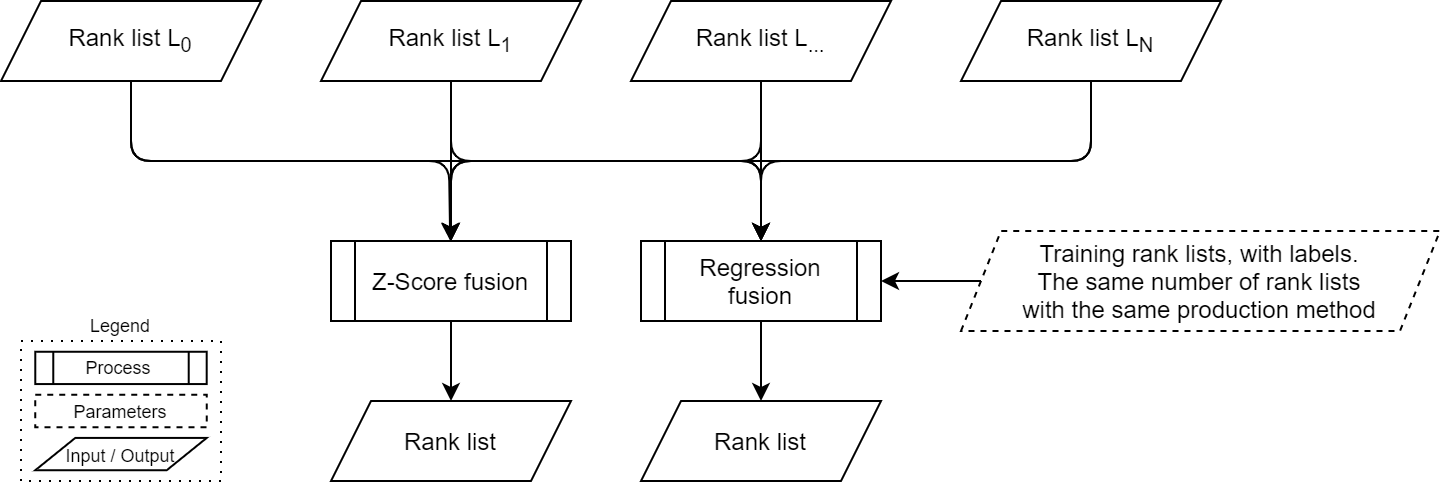
\includegraphics[width=1\linewidth]{img/schema-fusion.png}
\end{figure*}

\begin{table}
  \caption{Fusion evaluation summary, mean across every datasets}
  \label{tab:fusion_evaluation_summary}
  \resizebox{\linewidth}{!}{
  \begin{tabular}{l c c c}
    \toprule
                      & AP   & RPrec & HPrec \\
    \midrule
    Z-Score fusion    & 0.85 & 0.78   & 101.50 \\
    Regression fusion & 0.85 & 0.78   & 98.50  \\
    \midrule
    \textit{Individual methods average} & \textit{0.79} & \textit{0.71} & \textit{78.88} \\
    \bottomrule
  \end{tabular}
  }
\end{table}
